\begin{figure}[t]
    \vspace*{5pt}
    \centering
    % \begin{tabular}{c@{\hspace{1.5pt}}c@{\hspace{1.5pt}}}
    %\subfloat[Trajectories defined by 3 points \label{fig:3point}]{%
      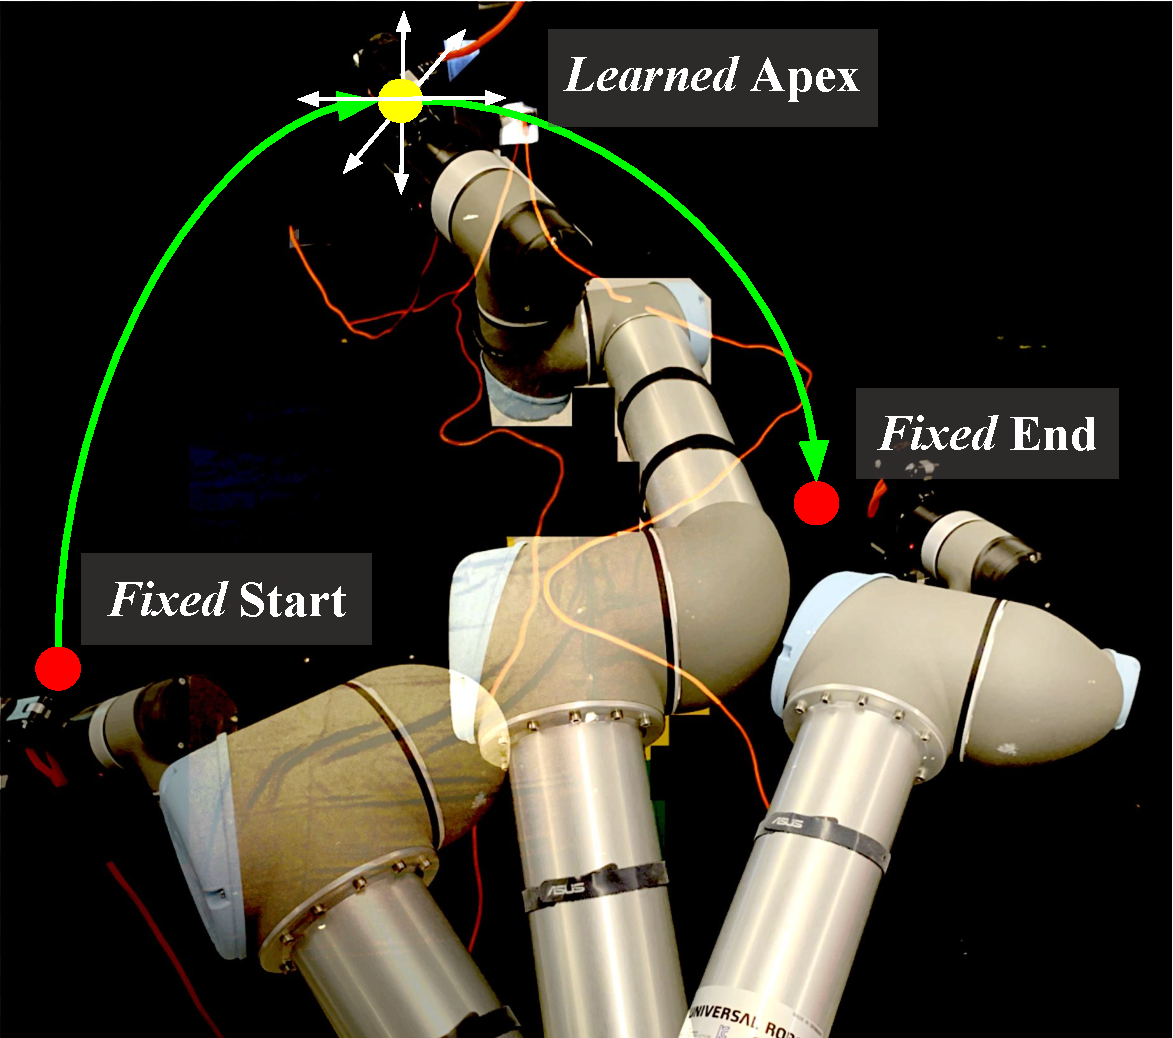
\includegraphics[height=110pt]{figures/3point.pdf}%}%
      \hfill
    %\subfloat[Physical space layout\label{fig:layout}]{%
      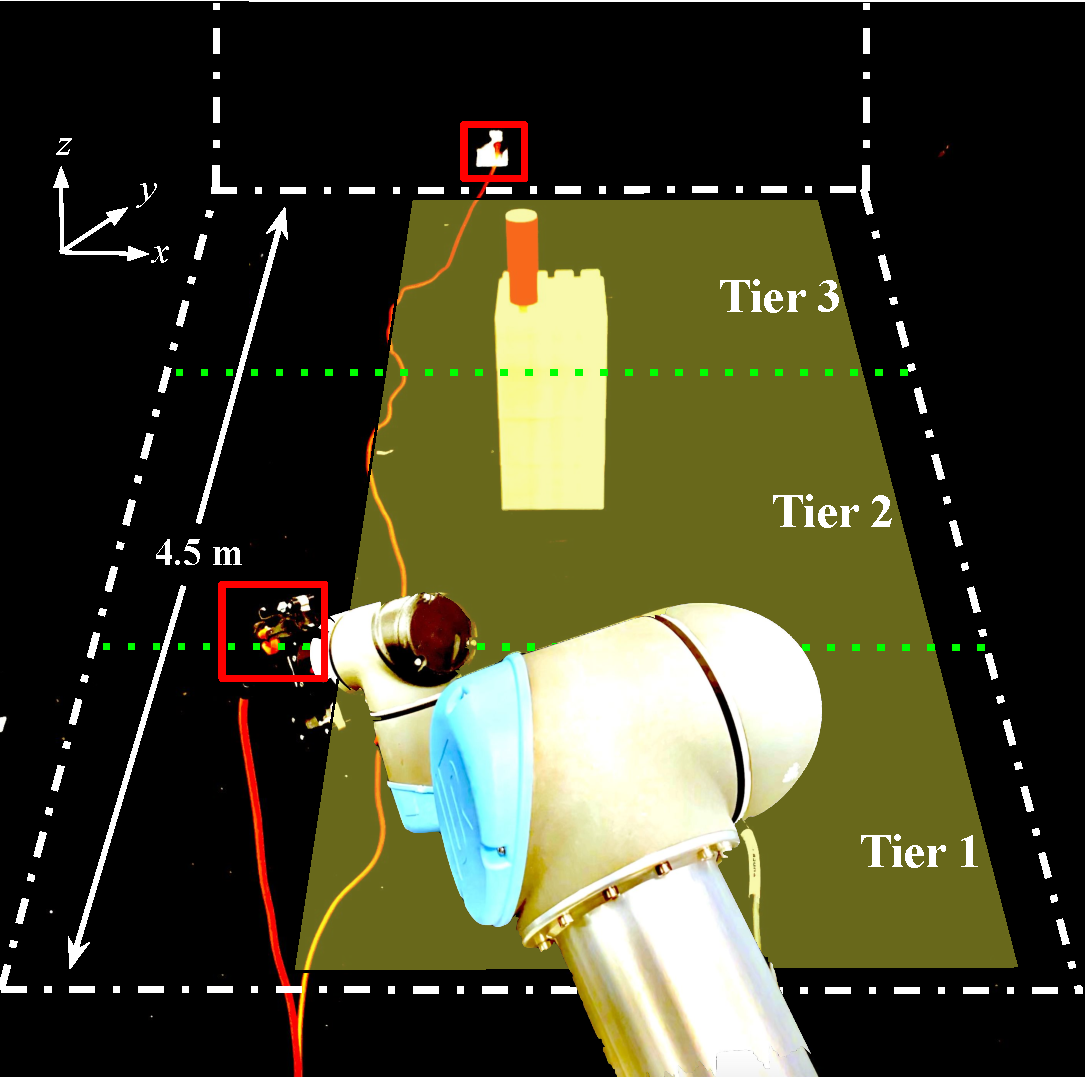
\includegraphics[height=110pt]{figures/layout_new.pdf}%}
    % \end{tabular}
    \caption{\textbf{Left: }Using three points in a curve to control the trajectory of the cable. The start and end points are fixed using the arm configurations. We change the trajectory by varying the apex configuration. \textbf{Right: }Design of physical experiments. We randomize the white Lego bricks’ location within the yellow shaded area. For vaulting and knocking, the width of the yellow area is 1.5~m, and 1.0~m for weaving. The yellow area is divided into three difficulty tiers.}
   % {\color{red} We need to change the label on the mid point.  Can you add arrows indicating that the mid point can by varied left/right and up/down (and in/out).  Also can you reverse the colors so that it starts/stops on red, and we vary the midpoint yellow.}}
    %    \vspace*{-10pt}
    \label{fig:motion_and_floor}
    \vspace*{-10pt}
\end{figure}